% \chapter{Fractures}
% \chapter{Introduction}
\vspace*{\fill}
\begin{figure}[hp!]%
\thispagestyle{empty}
    \centering%
    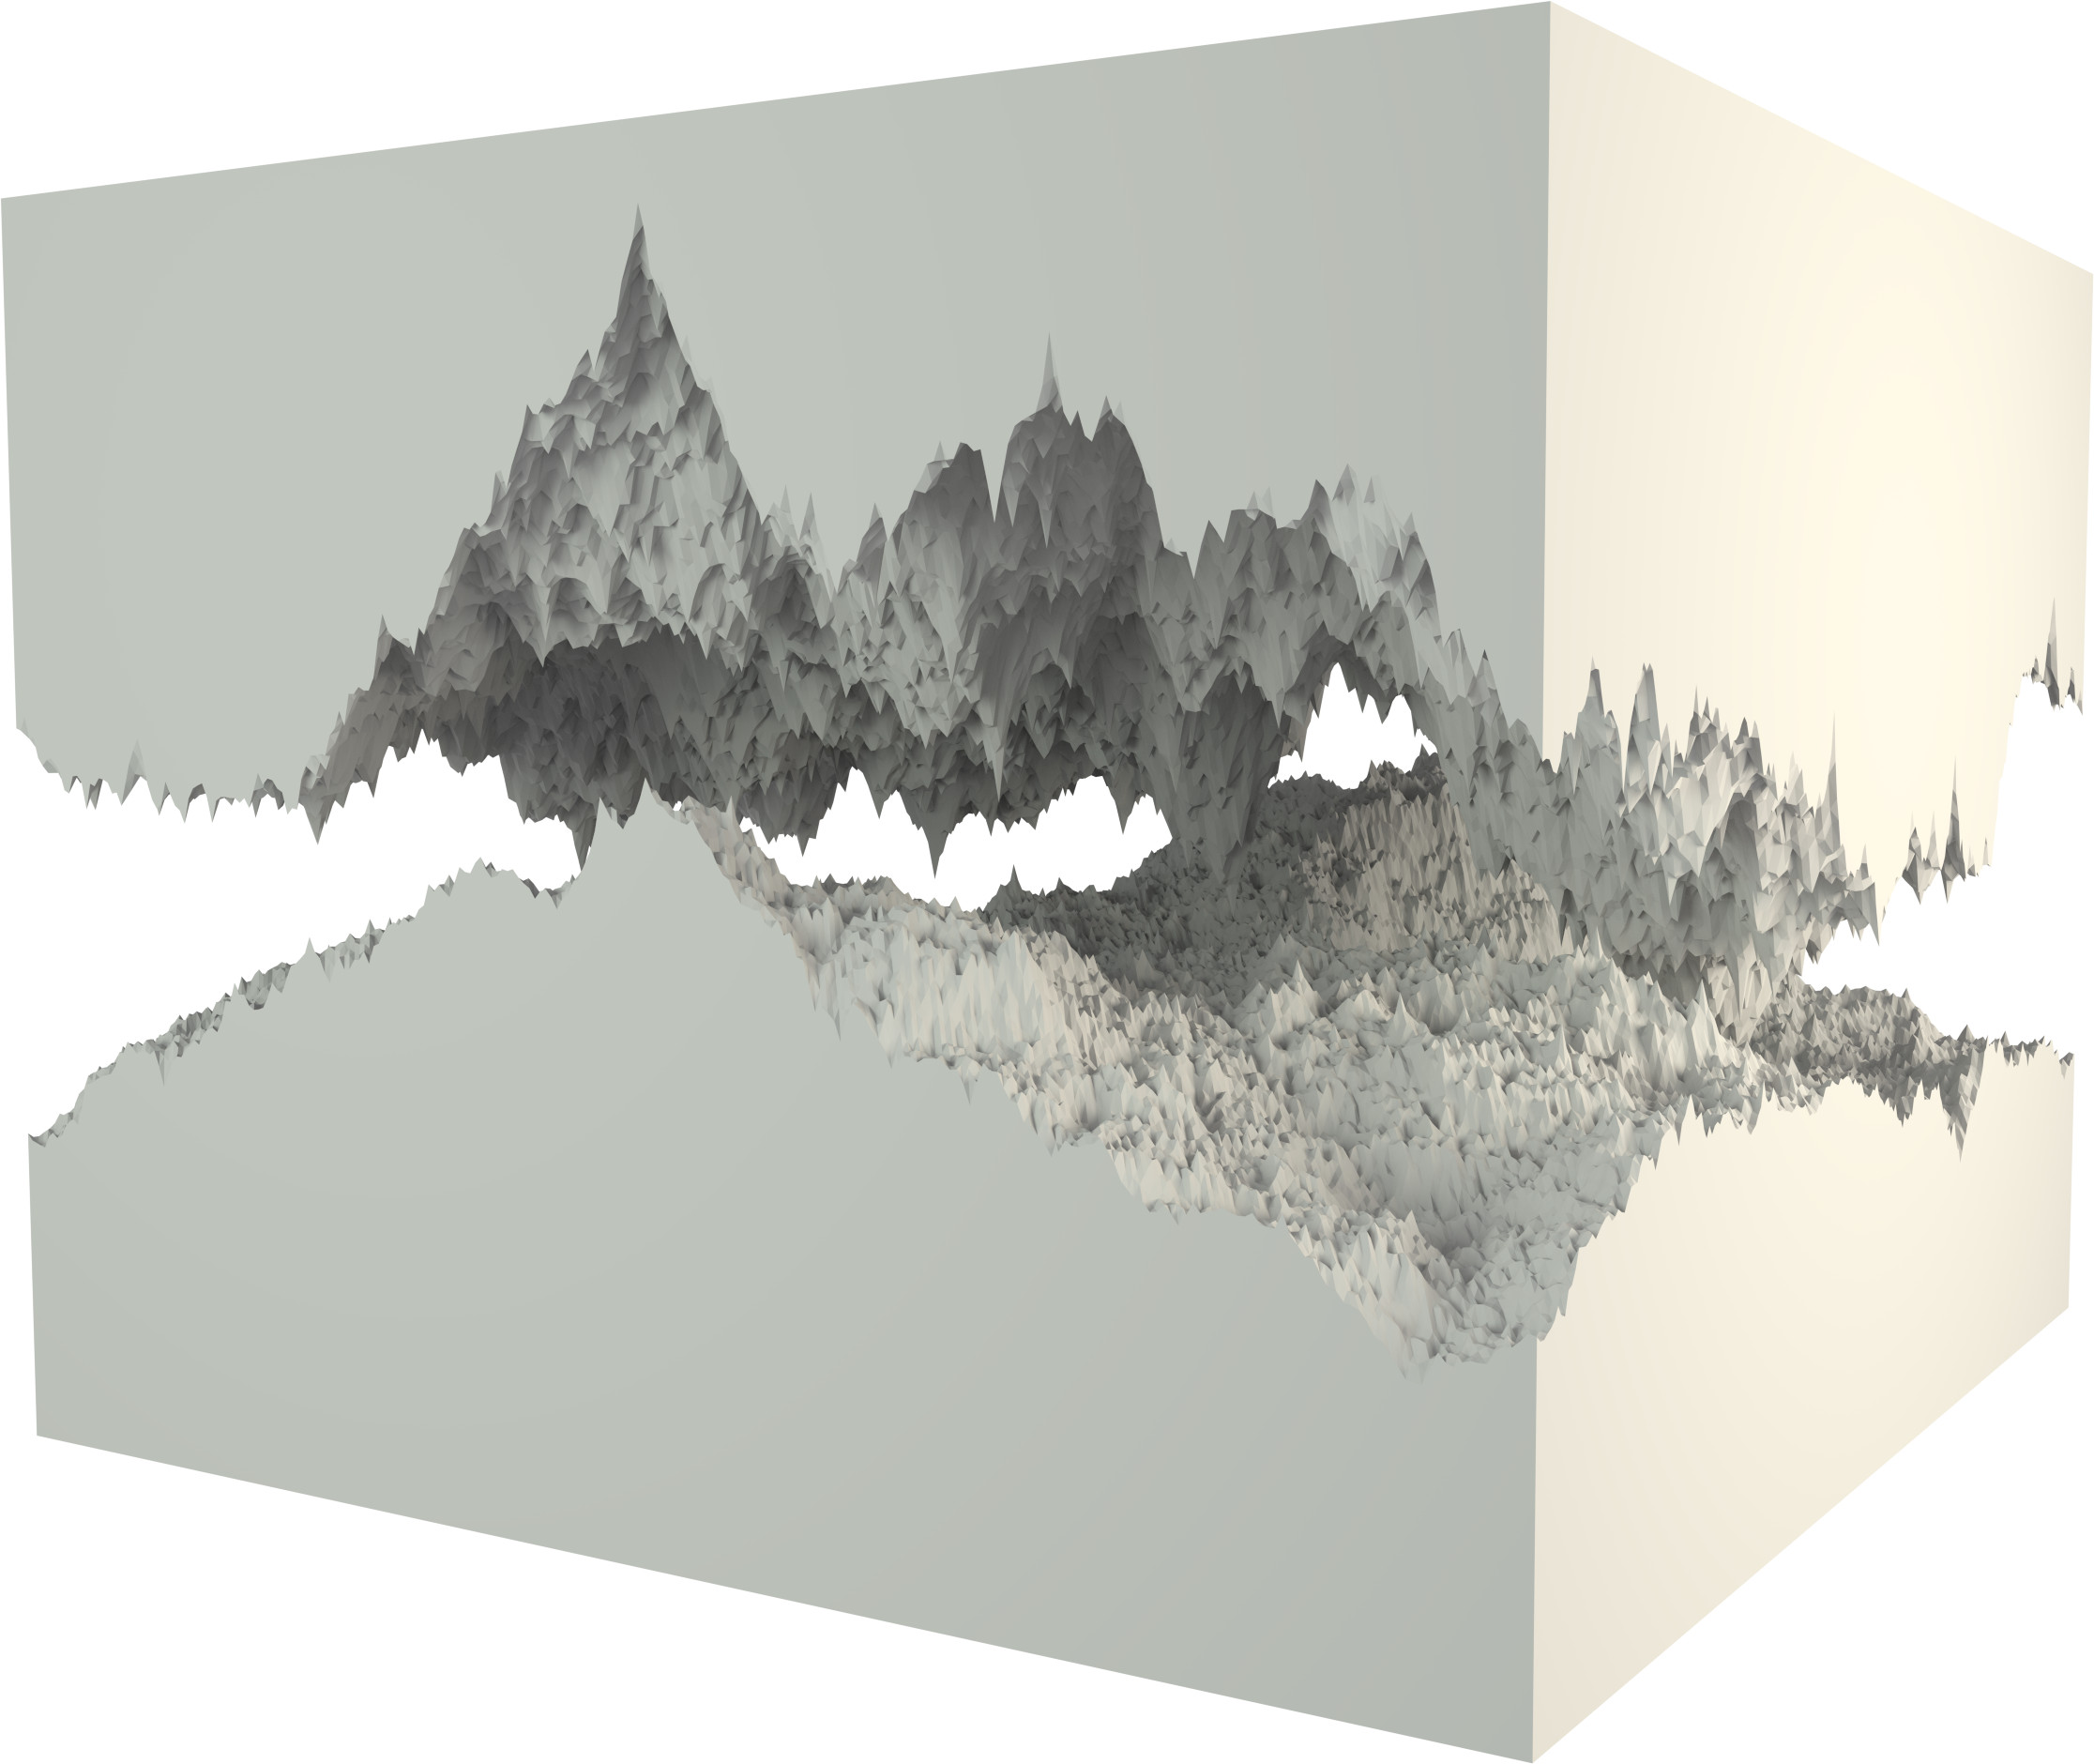
\includegraphics[width=\textwidth]{images/fracture/large_fracture05.jpg}%
    \caption{%
        A randomly generated fracture.%
    }%
\end{figure}%
\vspace{\fill}

\chapter*{Introduction}
\addcontentsline{toc}{chapter}{Introduction}
We want to study the behaviour of water trapped in nanoscale pores and fractures in silica, so need a way to generate and characterize such structures. We choose to model a fracture as two surfaces, with the volume between the surfaces as the void fraction. This makes it easier to make fractures, since we only need to create two surfaces to get a fracture. 

To generate realistic surfaces we could have used scans of the structures we want to simulate, but the problem with this approach is that the resulting fracture will depend a lot on how we interpret the image, and that we can not easily generate a lot of samples of surfaces. To avoid this we use fractals to describe surfaces, and use this to randomly generate surfaces and fractures that are statistically similar to real fractures. Like a lot of phenomena in nature, fractures and surfaces can be very well described by the theory of fractals\cite{mandelbrot1983fractal}, so we think that this method should give good results.

What makes a \emph{fractal} fractal, or what characterizes a fractal, does not have a rigorous definition, but in general a fractal is something that looks similar to itself at different length scales. A fractal might be \emph{identical} to itself at different length-scales (self-similar), or be \emph{statistically similar} to itself (statistically self-similar). In one dimension this looks like \todoao{Examples of 1D, scale x and y equally for self-similar, different scaling for self-affine}

% Fractals and concepts similar to fractals have been discussed as early as the 17th century, but the use of fractals in natural sciences didn't really \hl{take off} before computers became \hl{readily} available and Benoit Mandelbrot gathered and developed a lot of theory on fractals in ``The Fractal Geometry of Nature''\cite{mandelbrot1983fractal}. 

% \todoa{Define fractal dimension}
\todoao{More intro about fractals, some history?}
% \tododone{Define fractal, define self-similarirt and similar terms}

% \todoao{change wording? copied from Fractals...}
% An \emph{affine transformation} transforms a point $\bvec x = (x_1, \dots, x_n)$ into new points $\bvec x' = (r_1x_1, \dots, r_n, x_n)$, where the scaling rations $r_1, \dots, r_n$ are \emph{not} all equal.
% 
% A bounded set $\mathcal{S}$ is \emph{self-affine} if $\mathcal{S}$ is the union of $N$ non-overlapping subsets $\mathcal{S}_1, \dots, \mathcal{S}_N$, each of which is congruent to the set $\bvec r(\mathcal{S})$ obtained from $\mathcal S$ by the affine transform defined by $\bvec r$. Here \emph{congruent} means that the set of points $\mathcal{S}$ is identical to the set of points $\bvec r(\mathcal{S})$ after possible translations and/or rotations of the set\cite{feder1988fractals}.
% 
% A set $\mathcal{S}$ is \emph{statistically self-affine} if $\mathcal{S}$ is the union of $N$ non-overlapping subsets each of which is scaled down by $\bvec r$ from the original, and is identical in all statistical respects to $\bvec r(\mathcal{S})$.

\chapter{Fractals and fractures}
\todoao{Finish fractals and fractures chapter thing}%
%
% \section{Surface area}
% \section{Distance to nearest atom}
% \begin{itemize}
%     \item Fractals
%     \item Fractional Brownian Motion
%     \item The Hurst Exponent
% \end{itemize}
To generate a fractal surface we use fractional Brownian motion (fBm), introduced by Mandelbrot and van Ness in 1968\cite{mandelbrot1968fractional}. Fractional Brownian motion is a generalization of Brownian motion, which is the random motion of particles suspended in a fluid, which comes from their collisions with the atoms and molecules in the fluid. 

Fractional Brownian motion is a process that generates data that is fractal, in the sense that it is self-similar. The data generated by this process can be characterized by a parameter denoted $H$, often called the Hurst exponent. $H$ is related to the autocorrelation (define?) of a data set, and is always a number between 0 and 1. It has been shown that fractures and other phenomena in nature have a Hurst exponent of around 0.75, for over eleven decades of length scales\cite{renard2013hurst}, so we will try to generate fractures with this Hurst exponent for our simulations.\todoco{No real fractals in nature, since limited resolution?}
%It is directly related to the fractal dimension $D$ via\cite{feder1988fractals}\todoao{The Hurst exponent relates the root mean square value of the change $dy$ to the distance $x$ over which it changes}
% \begin{align*}
%     D = d - H
% \end{align*}

\hl{The Hurst exponent quantifies the relative tendency of a data set to either regress to the mean, or to cluster in a direction.} $H\in[0,0.5]$ indicates a dataset with long-term switching between high and low values in adjacent pairs, meaning that a single high value will probably be followed by a low value, and vice versa. $H\in[0.5,1.0]$ indicates a \hl{time series} with long-term positive autocorrelation, meaning both that a high value will probably be followed by another high value, and that the values a long time into the future will also tend to be \hl{high (increasing?)}.\todoao{Remove this, or rewrite!}

Samples of fBm with different Hurst parameters will differ in what can quantitatively be called the ``roughness'' or the ``randomness'' of the data, as can be seen in \cref{fig:fBm_examples}, where we have plotted some samples of fBm with different Hurst exponents.

% \todo{in honor of both Harold Edwin Hurst and Ludwig Otto H\"older}

The Hurst exponent and the use of it as a means of characterizing a dataset was developed in the field of hydrology, as seen in \cite{hurst1951longterm,hurst1965longterm}, where it was used to determine the optimal dam sizing for the Nile river's, by studying the large fluctuations in the flow rate of the river, which there are extensive records of\todoco{rewrite this one-sentence paragraph}. The exponent is denoted $H$ in honor of both Harold Hurst, who was the lead researcher in these studies, and in honor of Otto H\"older.\todoco{Why holder?}
%
% \todobo{See \cite{mu1988steel} for ref. on fractal dimension of fractured steel surface}%
% \todob{No true fractals in nature, since we need infinite resolution. $H = $ Hausdorff dimension? index-$\alpha$?}%
% \todob{Decide on which Hurst figure, and maybe resize the label box in alt. 1? (just increase fig size in plot script)}%
%
\begin{figure}[htpb]%
    \centering%
    {%
%         \newcommand{\s}{\sim}%
        \newcommand{\sa}{H $\approx$ }%
        \includesvg[width=0.8\textwidth, svgpath = ./images/Hurst/]{fbm_1d_examples_grid01}%
    }%
    \caption{%
        Samples of fractional Brownian motion (fBm) with different Hurst exponents, generated using the built-in Matlab function \mono{wfbm}, which uses uses a wavelet-based synthesis method\cite{abry1996wavelet} for generating fBm.%
    }%
    \label{fig:fBm_examples}%
\end{figure}%
